\documentclass[tikz,border=8pt]{standalone}
% Shared look for every TikZ diagram. Load with % Shared look for every TikZ diagram. Load with % Shared look for every TikZ diagram. Load with \input{../../tools/tikz-style.tex}
\usepackage[T1]{fontenc}
\usepackage{lmodern}
\renewcommand{\sfdefault}{lmr}  % diagrams use the same serif as the text
\usetikzlibrary{arrows.meta, positioning, shapes.geometric, calc, fit, backgrounds}
\definecolor{cblue}{HTML}{4C78A8}
\definecolor{corange}{HTML}{F58518}
\definecolor{cgreen}{HTML}{54A24B}
\definecolor{cred}{HTML}{E45756}
\definecolor{cpurple}{HTML}{B279A2}
\definecolor{cgrey}{HTML}{6B6B6B}
\tikzset{
  every picture/.style={font=\sffamily, line width=1.2pt},
  box/.style={draw=#1, fill=#1!12, rounded corners=4pt, align=center, inner sep=7pt, minimum height=1.1cm},
  box/.default=cgrey,
  arrow/.style={-{Stealth[length=3mm]}, draw=cgrey, line width=1.4pt},
  title/.style={font=\sffamily\bfseries\Large},
  note/.style={font=\sffamily\small, text=cgrey, align=center},
}
\AtBeginDocument{\hyphenpenalty=10000 \exhyphenpenalty=10000}

\usepackage[T1]{fontenc}
\usepackage{lmodern}
\renewcommand{\sfdefault}{lmr}  % diagrams use the same serif as the text
\usetikzlibrary{arrows.meta, positioning, shapes.geometric, calc, fit, backgrounds}
\definecolor{cblue}{HTML}{4C78A8}
\definecolor{corange}{HTML}{F58518}
\definecolor{cgreen}{HTML}{54A24B}
\definecolor{cred}{HTML}{E45756}
\definecolor{cpurple}{HTML}{B279A2}
\definecolor{cgrey}{HTML}{6B6B6B}
\tikzset{
  every picture/.style={font=\sffamily, line width=1.2pt},
  box/.style={draw=#1, fill=#1!12, rounded corners=4pt, align=center, inner sep=7pt, minimum height=1.1cm},
  box/.default=cgrey,
  arrow/.style={-{Stealth[length=3mm]}, draw=cgrey, line width=1.4pt},
  title/.style={font=\sffamily\bfseries\Large},
  note/.style={font=\sffamily\small, text=cgrey, align=center},
}
\AtBeginDocument{\hyphenpenalty=10000 \exhyphenpenalty=10000}

\usepackage[T1]{fontenc}
\usepackage{lmodern}
\renewcommand{\sfdefault}{lmr}  % diagrams use the same serif as the text
\usetikzlibrary{arrows.meta, positioning, shapes.geometric, calc, fit, backgrounds}
\definecolor{cblue}{HTML}{4C78A8}
\definecolor{corange}{HTML}{F58518}
\definecolor{cgreen}{HTML}{54A24B}
\definecolor{cred}{HTML}{E45756}
\definecolor{cpurple}{HTML}{B279A2}
\definecolor{cgrey}{HTML}{6B6B6B}
\tikzset{
  every picture/.style={font=\sffamily, line width=1.2pt},
  box/.style={draw=#1, fill=#1!12, rounded corners=4pt, align=center, inner sep=7pt, minimum height=1.1cm},
  box/.default=cgrey,
  arrow/.style={-{Stealth[length=3mm]}, draw=cgrey, line width=1.4pt},
  title/.style={font=\sffamily\bfseries\Large},
  note/.style={font=\sffamily\small, text=cgrey, align=center},
}
\AtBeginDocument{\hyphenpenalty=10000 \exhyphenpenalty=10000}

\begin{document}
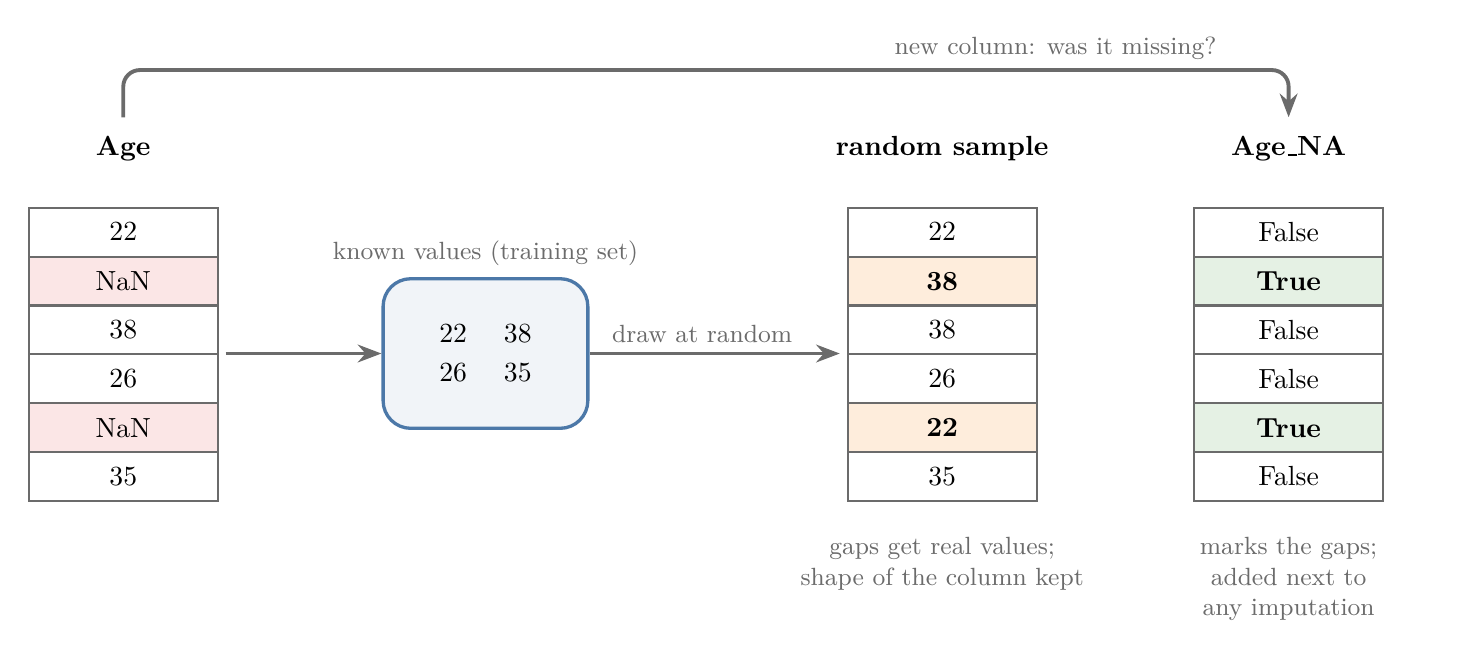
\begin{tikzpicture}
  % one Age column with two gaps, handled two ways
  \newcommand{\col}[3]{% #1 x, #2 title, #3 list of cells (text/colour)
    \node[font=\sffamily\bfseries] at (#1,0.75) {#2};
    \foreach \t/\c [count=\i] in {#3} {
      \node[draw=cgrey, fill=\c!15, minimum width=2.4cm, minimum height=0.62cm, line width=0.8pt]
        at (#1,-\i*0.62+0.31) {\t};
    }
  }
  \col{0}{Age}{22/white, NaN/cred, 38/white, 26/white, NaN/cred, 35/white}
  % the bag of known values
  \node[draw=cblue, fill=cblue!8, rounded corners=10pt, minimum width=2.6cm, minimum height=1.9cm,
        align=center] (bag) at (4.6,-1.85) {22 \quad 38\\[2pt] 26 \quad 35};
  \node[note, anchor=south] at (bag.north) {known values (training set)};
  \col{10.4}{random sample}{22/white, \textbf{38}/corange, 38/white, 26/white, \textbf{22}/corange, 35/white}
  \col{14.8}{Age\_NA}{False/white, \textbf{True}/cgreen, False/white, False/white, \textbf{True}/cgreen, False/white}
  \draw[arrow] (1.3,-1.85) -- (bag.west);
  \draw[arrow] (bag.east) -- node[above, note, pos=0.45] {draw at random} (9.1,-1.85);
  \draw[arrow, rounded corners=6pt] (0,1.15) -- (0,1.75) -- node[above, note, pos=0.8] {new column: was it missing?} (14.8,1.75) -- (14.8,1.15);
  \node[note, text width=4cm, anchor=north] at (10.4,-4.05) {gaps get real values;\\ shape of the column kept};
  \node[note, text width=3.6cm, anchor=north] at (14.8,-4.05) {marks the gaps;\\ added next to any imputation};
\end{tikzpicture}
\end{document}
